\que{Закон изменения количества движения. Интегральная  форма   уравнения движения. Внутренние и внешние силы. Массовые и поверхностные силы. }

\paragraph{Закон изменения количества движения.} 
\begin{definition*}
	Вектор 
	\begin{equation*}
		\mathbf{I} = \int\limits_{V} \mathbf{v} \, dm = \int\limits_{V} \rho \mathbf{v} \, dV,
	\end{equation*}
	называют вектором \textit{количества движения} (или импульса) сплошной среды.
\end{definition*}

\begin{axiom}[закон изменения количества движения]
	Для любых двух сплошных сред $\mathcal{B}$ и $\mathcal{B}_1$ в любой момет времени $t$ существует векторная функция $\mathcal{F} = \mathcal{F}(\mathcal{B}, \mathcal{B}_1, t)$, возможно ноль-значная (т.е. $\mathcal{F} = \mathbf{0}$), называемая \textbf{вектором силы} взаимодействия тел $\mathcal{B}$ и $\mathcal{B}_1$ и обладающая следующими свойствами:
	\begin{enumerate}
		\item аддитивностью:
		\begin{align*}
			\mathcal{F}(\mathcal{B}' + \mathcal{B}'', \mathcal{B}_1, t) &= \mathcal{F}(\mathcal{B}', \mathcal{B}, t) + \mathcal{F}(\mathcal{B}'', \mathcal{B}_1, t), \\
			\mathcal{F}(\mathcal{B}, \mathcal{B}'_1 + \mathcal{B}''_1, t) &= \mathcal{F}(\mathcal{B}, \mathcal{B}'_1, t) + \mathcal{F}(\mathcal{B}, \mathcal{B}''_1, t),
		\end{align*}
		где $\mathcal{B} = \mathcal{B}' \cup \mathcal{B}'', \quad \mathcal{B}_1 = \mathcal{B}'_1 \cup \mathcal{B}''_1$.
		
		\item скорость изменения вектора количества движения $\mathbf{I}$ сплошной среды $\mathcal{B}$ в любой момент времени $t$ равна вектору $\mathcal{F}(\mathcal{B}, t) = \mathcal{F}(\mathcal{B}, \mathcal{B}^{e}, t)$ --- \textbf{суммарному вектору внешних сил}, действующих на тело $\mathcal{B}$ ($\mathcal{B}^{e} = \mathcal{U} \ \mathcal{B}$ --- внешность тела $\mathcal{B}$):
		\begin{equation*}
			d\mathbf{I} / dt = \mathcal{F}.
		\end{equation*}
	\end{enumerate}
	
	Последнее соотношение называют \textbf{законом изменения количества движения} (законом изменения импульса).
\end{axiom}

\begin{definition*}
	\textit{Плотностью массовых сил} называют вектор $\mathbf{f}$:
	\begin{equation*}
		\mathbf{f} = \frac{d\mathcal{F}}{dm} = \frac{d\mathcal{F}}{\rho dV},
	\end{equation*}
	а \textit{плотностью поверхностных сил} называют вектор $\mathbf{s}$:
	\begin{equation*}
		\mathbf{s} = d\mathcal{F} / d\Sigma,
	\end{equation*}
	здесь $dm$ --- масса элементарного объема сплошной среды $dV$.
	
	
	В силу свойства аддитивности $\mathcal{F}$, имеют место следующие соотношения для всего объема сплошной среды, занимающей объем $V$ в $\mathcal{K}$:
	\begin{gather*}
		\mathcal{F} = \mathcal{F}_m + \mathcal{F}_{\Sigma}, \\
		\mathcal{F}_m = \int\limits_{V} \mathbf{f} \, dm = \int\limits_{V} \rho \mathbf{f} \, dV, \quad \mathcal{F}_{\Sigma} = \int\limits_{\Sigma} \mathbf{s} \, d\Sigma.
	\end{gather*}
	
	Вектор $\mathcal{F}_m$ называют \textit{суммарным вектором внешних массовых сил}, действующих на рассматриваемую сплошную среду, а $\mathcal{F}_{\Sigma}$ --- \textit{суммарным вектором внешних поверхностных сил}.
\end{definition*}

С учетом перечисленных выше соотношений закон иззменения количества движения можно записать в \textit{интегральной форме}:
\begin{equation*}
	\frac{d}{dt} \int\limits_{V} \rho \mathbf{v} \, dV = \int\limits_{V} \rho \mathbf{f} \, dV + \int\limits_{\Sigma} \mathbf{s} \, d\Sigma.
\end{equation*}

\paragraph{Внешние и внутренние силы. Массовые и поверхностные силы.} Массовые $\mathbf{f}$ и поверхностные $\mathbf{s}$ силы являются \textit{внешними} силами по отношению к объему сплошной среды $V$, так как они вызваны объектами, не принадлежащими к данному объему $V$ сплошной среды (внешними объектами). 

Основными видами внешних массовых сил являются: 
\begin{enumerate}
	\item сила тяжести $\mathbf{f} = g_{\Sigma} \bar{\mathbf{e}}$, где $g_{\Sigma}$ --- ускорение свободного падения на поверхности планеты, а $\bar{\mathbf{e}}$ --- вектор нормали к поверхности планеты;
	
	\item внешние силы инерции, вызванные движением тела по отношению к подвижной системе отсчета;
	
	\item электромагнитные силы. 
\end{enumerate}

Внешние поверхностные силы --- это силы взаимодействия двух контактирующих друг с другом сплошных среж, например, одного твердого тела с другим при ударе. 

Кроме внешних сил в механике сплошной среды существуют также понятие \textit{внутренних сил}. Пользуясь правилом дифференцирования интеграла по подвижному объему и используя уравнение неразрывности в Эйлеровом описании, преобразуем закон изменения количества движения в интегральной форме:
\begin{align*}
	\frac{d}{dt} \int\limits_{V} \rho \mathbf{v} \, dV &= \int\limits_{V}\left(\frac{\partial}{\partial t} \rho \mathbf{v} + \nabla \cdot \left(\rho \mathbf{v} \otimes \mathbf{v}\right)\right) \, dV = \\
	&= \int\limits_{V} \left(\frac{\partial \rho}{\partial t} \mathbf{v} + \rho \frac{\partial \mathbf{v}}{\partial t} + (\nabla \cdot \rho \mathbf{v}) \mathbf{v} + \rho \mathbf{v} \cdot \nabla \otimes \mathbf{v}\right) \, dV = \int\limits_{V} \rho \frac{d \mathbf{v}}{d t} \, dV.
\end{align*}

Тогда получаем: 
\begin{equation*} \tag{$\ast$} \label{omega}
	\Omega = \int\limits_{V} \rho \left(\mathbf{f} - \frac{d \mathbf{v}}{dt}\right) \, dV + \int\limits_{\Sigma} \mathbf{s} \, d\Sigma = 0.
\end{equation*}

Отюда следует, что ускорение $(d \mathbf{v} / dt)$ представляет собой плотность некоторых \textit{массовых сил}, но уже \textit{внутренних}, вызванных инерционными эффектами, поэтому их еще называют \textit{внутренними инерционными силами}. 

Рассмотрим пример \textit{внутренних поверхностных сил}. 

\begin{wrapfigure}[17]{r}{0.5\textwidth}
	\centering
	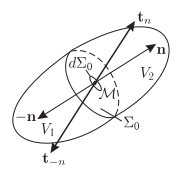
\includegraphics[width=0.7\linewidth]{img/que16}
	\caption{Внутренние поверхностные силы на площадке $\Sigma_0$}
	\label{fig:que16}
\end{wrapfigure}


Произвольную область $V$ разделим на две части $V_1$ и $V_2$ поверхностью $\Sigma_0$. Вектор нормали в точке $\mathcal{M}$ обозначим как $\mathbf{n}$, если он направлен в сторону $V_1$. На области $V_1$ и $V_2$ жействуют суммарные векторы внешних сил $\mathcal{F}_1$ и $\mathcal{F}_2$. Если рассмотреть элементарную площадку $d\Sigma \in \Sigma_0$, которой принадлежит рассматриваемая точка, то на ней действует поверхностная сила $d\mathcal{F}_1$ для области $V_1$ и $d\mathcal{F}_2$ для $V_2$. Обозначим плотности этих сил следующим образом:
\begin{equation*}
	\mathbf{t}_{n} = d\mathcal{F}_1 / d\Sigma \quad \text{и} \quad t_{-n} = d\mathcal{F}_2 / d\Sigma.
\end{equation*} 

Векторы $\mathbf{t}_n$ и $\mathbf{t}_{-n}$ называют \textit{векторами напряжений}, они представляют собой плотности \textit{внутренних поверхностных сил} по отношению ко всей области $V$ сплошной среды (так как они определены для внутренних точек $\mathcal{M}$ этой области).
